% 
% Annual Cognitive Science Conference
% Sample LaTeX Paper -- Proceedings Format
% 

% Original : Ashwin Ram (ashwin@cc.gatech.edu)       04/01/1994
% Modified : Johanna Moore (jmoore@cs.pitt.edu)      03/17/1995
% Modified : David Noelle (noelle@ucsd.edu)          03/15/1996
% Modified : Pat Langley (langley@cs.stanford.edu)   01/26/1997
% Latex2e corrections by Ramin Charles Nakisa        01/28/1997 
% Modified : Tina Eliassi-Rad (eliassi@cs.wisc.edu)  01/31/1998
% Modified : Trisha Yannuzzi (trisha@ircs.upenn.edu) 12/28/1999 (in process)
% Modified : Mary Ellen Foster (M.E.Foster@ed.ac.uk) 12/11/2000
% Modified : Ken Forbus                              01/23/2004
% Modified : Eli M. Silk (esilk@pitt.edu)            05/24/2005
% Modified: Niels Taatgen (taatgen@cmu.edu) 10/24/2006

%% Change ``a4paper'' in the following line to ``letterpaper'' if you are
%% producing a letter-format document.

\documentclass[10pt,letterpaper]{article}
\usepackage{graphicx}
\usepackage{cogsci}
\usepackage{pslatex}
\usepackage{apacite}


\title{The Pragmatics of Metaphor Understanding: A Computational Approach}
 
\author{{\large \bf Justine T. Kao (justinek@stanford.edu)} \\
  Department of Psychology\\
  Stanford, CA, USA
  \AND {\large \bf Noah D. Goodman (ngoodman@stanford.edu)} \\
  Department of Psychology\\
  Stanford, CA, USA}


\begin{document}

\maketitle


\begin{abstract}
Abstract goes here.
%Metaphor understanding has been widely studied in psychology, linguistics, philosophy, and computer science. One account of metaphor understanding is pragmatics. Some metaphor interpretations arise from pragmatics. Here we present a computational model of pragmatics that accounts for 

\textbf{Keywords:} 
language understanding; metaphor; pragmatics; computational models
\end{abstract}


\section{Introduction}
Brief description of the importance of metaphor.
Describe different approaches to studying metaphor understanding (cognitive, linguistic, relevance theory, etc). Zoom into approaches that emphasize pragmatics. 

Motivate need to formalize theories of pragmatic metaphor understanding using computational models. Describe rational speech act models on a high level and how they can be naturally extended to non-literal language understanding such as metaphor. Main ideas to introduce and motivate:

\begin{itemize} 
\item[(1)] Metaphor understanding involves prior knowledge of source and target 
\item[(2)] Metaphor interpretation driven by context and question under discussion 
\item[(3)] Metaphors can sometimes communicate information more efficiently than literal statements and hence can be optimal and rational speech acts.
\end{itemize}

\section{Behavioral Experiments}
Outline the three different experiments and the purpose of each. 
\begin{itemize}
\item[]Experiment 1: elicit sets of common features for each animal category. 
\item[]Experiment 2: elicit priors for these features associated with animals and people. 
\item[]Experiment 3: measure people's interpretation of literal or metaphorical descriptions under different QUDs (implicit or explicit).
\end{itemize}
\subsection{Materials and Methods}

Describe details of each of the three experiments (how many subjects, materials, setup, etc).


\subsubsection{Results}
Show results from Experiment 3.
Questions: Where should results for Exp 1 and 2 go? Also, which is more important/interesting, Effect 1 or Effect 2?
\begin{itemize}
\item[] Effect 1: Metaphorical response introduces ambiguity regarding feature 1 but also communicates information about features 2 and 3. 
\item[] Effect 2: Explicit QUD changes interpretation and increases probability of the feature under discussion being true.
\end{itemize}
 
\begin{figure}[ht]
\begin{center}
\scalebox{0.4}{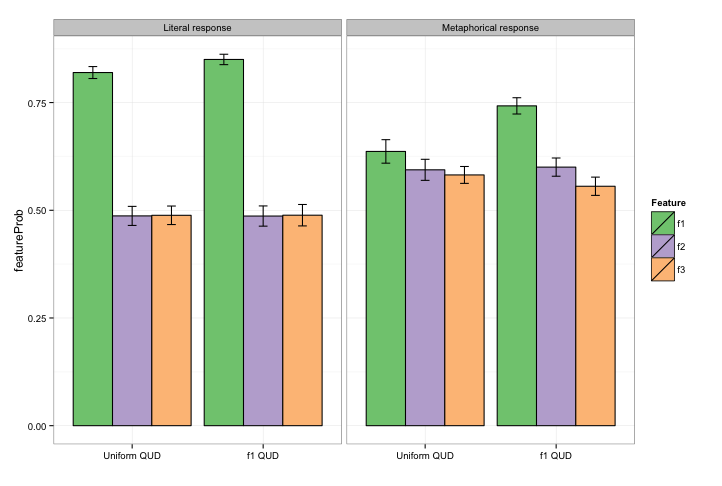
\includegraphics{Plots/exp1-temp.png}}
\end{center}
\caption{This is a figure.} 
\label{sample-figure}
\end{figure}


\section{Computational Model}
Introduce intuition for the model. Literal listener, recursive social reasoning, QUD and satisfaction of communicative goal, etc.

Lay out mathematical details of model.

Describe how priors from Experiment 2 get plugged into the model.
\subsection{Results}
Show qualitative results of model predictions: 
\begin{itemize}
\item[] Effect 1: The model interprets metaphors more ambiguously but makes inferences about additional features
\item[] Effect 2: Model interprets metaphors differently under different QUDs
\end{itemize}

\section{Model Comparison}
Compare model predictions to behavioral results. Scatter plot.

Compare with baseline models such as just animal prior or just human prior. Compare with baseline that does not have QUD.

\section{Discussion}
Discuss implication of results on the pragmatics of metaphor; discuss other effects we could explore using the modeling framework; suggest future directions.

\subsection{Footnotes}


\subsection{Tables}

\begin{table}[!ht]
\begin{center} 
\caption{Sample table title.} 
\label{sample-table} 
\vskip 0.12in
\begin{tabular}{ll} 
\hline
Error type    &  Example \\
\hline
Take smaller        &   63 - 44 = 21 \\
Always borrow~~~~   &   96 - 42 = 34 \\
0 - N = N           &   70 - 47 = 37 \\
0 - N = 0           &   70 - 47 = 30 \\
\hline
\end{tabular} 
\end{center} 
\end{table}


\subsection{Figures}

\begin{figure}[ht]
\begin{center}
\fbox{CoGNiTiVe ScIeNcE}
\end{center}
\caption{This is a figure.} 
\label{sample-figure}
\end{figure}


\section{Acknowledgments}

Place acknowledgments (including funding information) in a section at
the end of the paper.


\section{References}


\bibliographystyle{apacite}

\setlength{\bibleftmargin}{.125in}
\setlength{\bibindent}{-\bibleftmargin}

\bibliography{CogSci_Template}


\end{document}
